\documentclass[tikz,border=10pt]{standalone}
\usetikzlibrary{calc}
% Scale s = 0.021333 cm/px (from STYLE METRICS); y flipped
\begin{document}
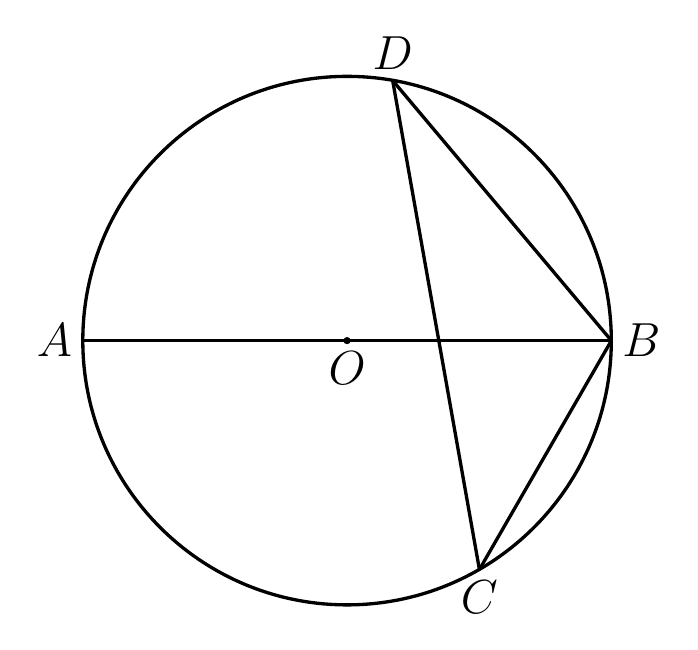
\begin{tikzpicture}[line join=round, line width=1.2pt]
  % Named coordinates (cm)
  \coordinate (O) at (0,0);
  \coordinate (A) at (-3.355,0);
  \coordinate (B) at (3.357,0);
  \coordinate (D) at (0.579,3.304);
  \coordinate (C) at (1.681,-2.907);
  \coordinate (X) at (1.162,0);

  % Circle of radius 157.28 px
  \draw (O) circle (3.356);

  % Diameter AB
  \draw (A) -- (B);

  % Chords BD, BC and segment DC
  \draw (B) -- (D);
  \draw (B) -- (C);
  \draw (D) -- (C);

  % Center dot
  \fill (O) circle (1.3pt);

  % Labels
  \node[left] at (A) {\fontsize{18}{21.6}\selectfont $A$};
  \node[right] at (B) {\fontsize{18}{21.6}\selectfont $B$};
  \node[above] at (D) {\fontsize{18}{21.6}\selectfont $D$};
  \node[below] at (C) {\fontsize{18}{21.6}\selectfont $C$};
  \node[below] at (O) {\fontsize{18}{21.6}\selectfont $O$};
\end{tikzpicture}
\end{document}